\chapter{Costruzione}

\section{Componenti}
Per autocostruire lo Spider Keyer sono necessari:
\begin{itemize}
	\item 1x Arduino Nano o clone
	\item 1x cicalino magnetico passivo 5 V
	\item 1x potenziometro lineare 10 $k\Omega$
	\item 1x connettore stereo 3.5 mm femmina
	\item 2x connettori RCA femmina
	\item 1x transistor NPN (T1), ad esempio BC337
	\item 2x fotoaccoppiatori (OK1 e OK2), ad esempio LTV816
	\item 1x condensatore elettrolitico (C3) da 10 $\mu F$ (16 V)
	\item 2x condensatori ceramici (C1 e C2) da 3.3 $nF$
	\item 2x induttanze (L1 e L2) da 100 $\mu H$
	\item 2x resistenze (R2 e R4) da 240 $\Omega$
	\item 1x resistenza (R3) da 100 $\Omega$
	\item 1x resistenza (R5) da 1 $k\Omega$.
\end{itemize}

I valori dei componenti passivi non sono critici: \`e possibile utilizzare valori simili senza incorrere in malfunzionamenti.

\begin{samepage}
	Se si usa un cicalino attivo, eliminare T1, C3 e R5 e creare un ponte tra il cicalino e il pin D11 dell'Arduino (a sinistra nella figura). In ogni caso \`e consigliato verificare nel datasheet del cicalino che sia in grado di generare toni della frequenza desiderata (in genere sotto 1 $kHz$).
	\begin{center}
		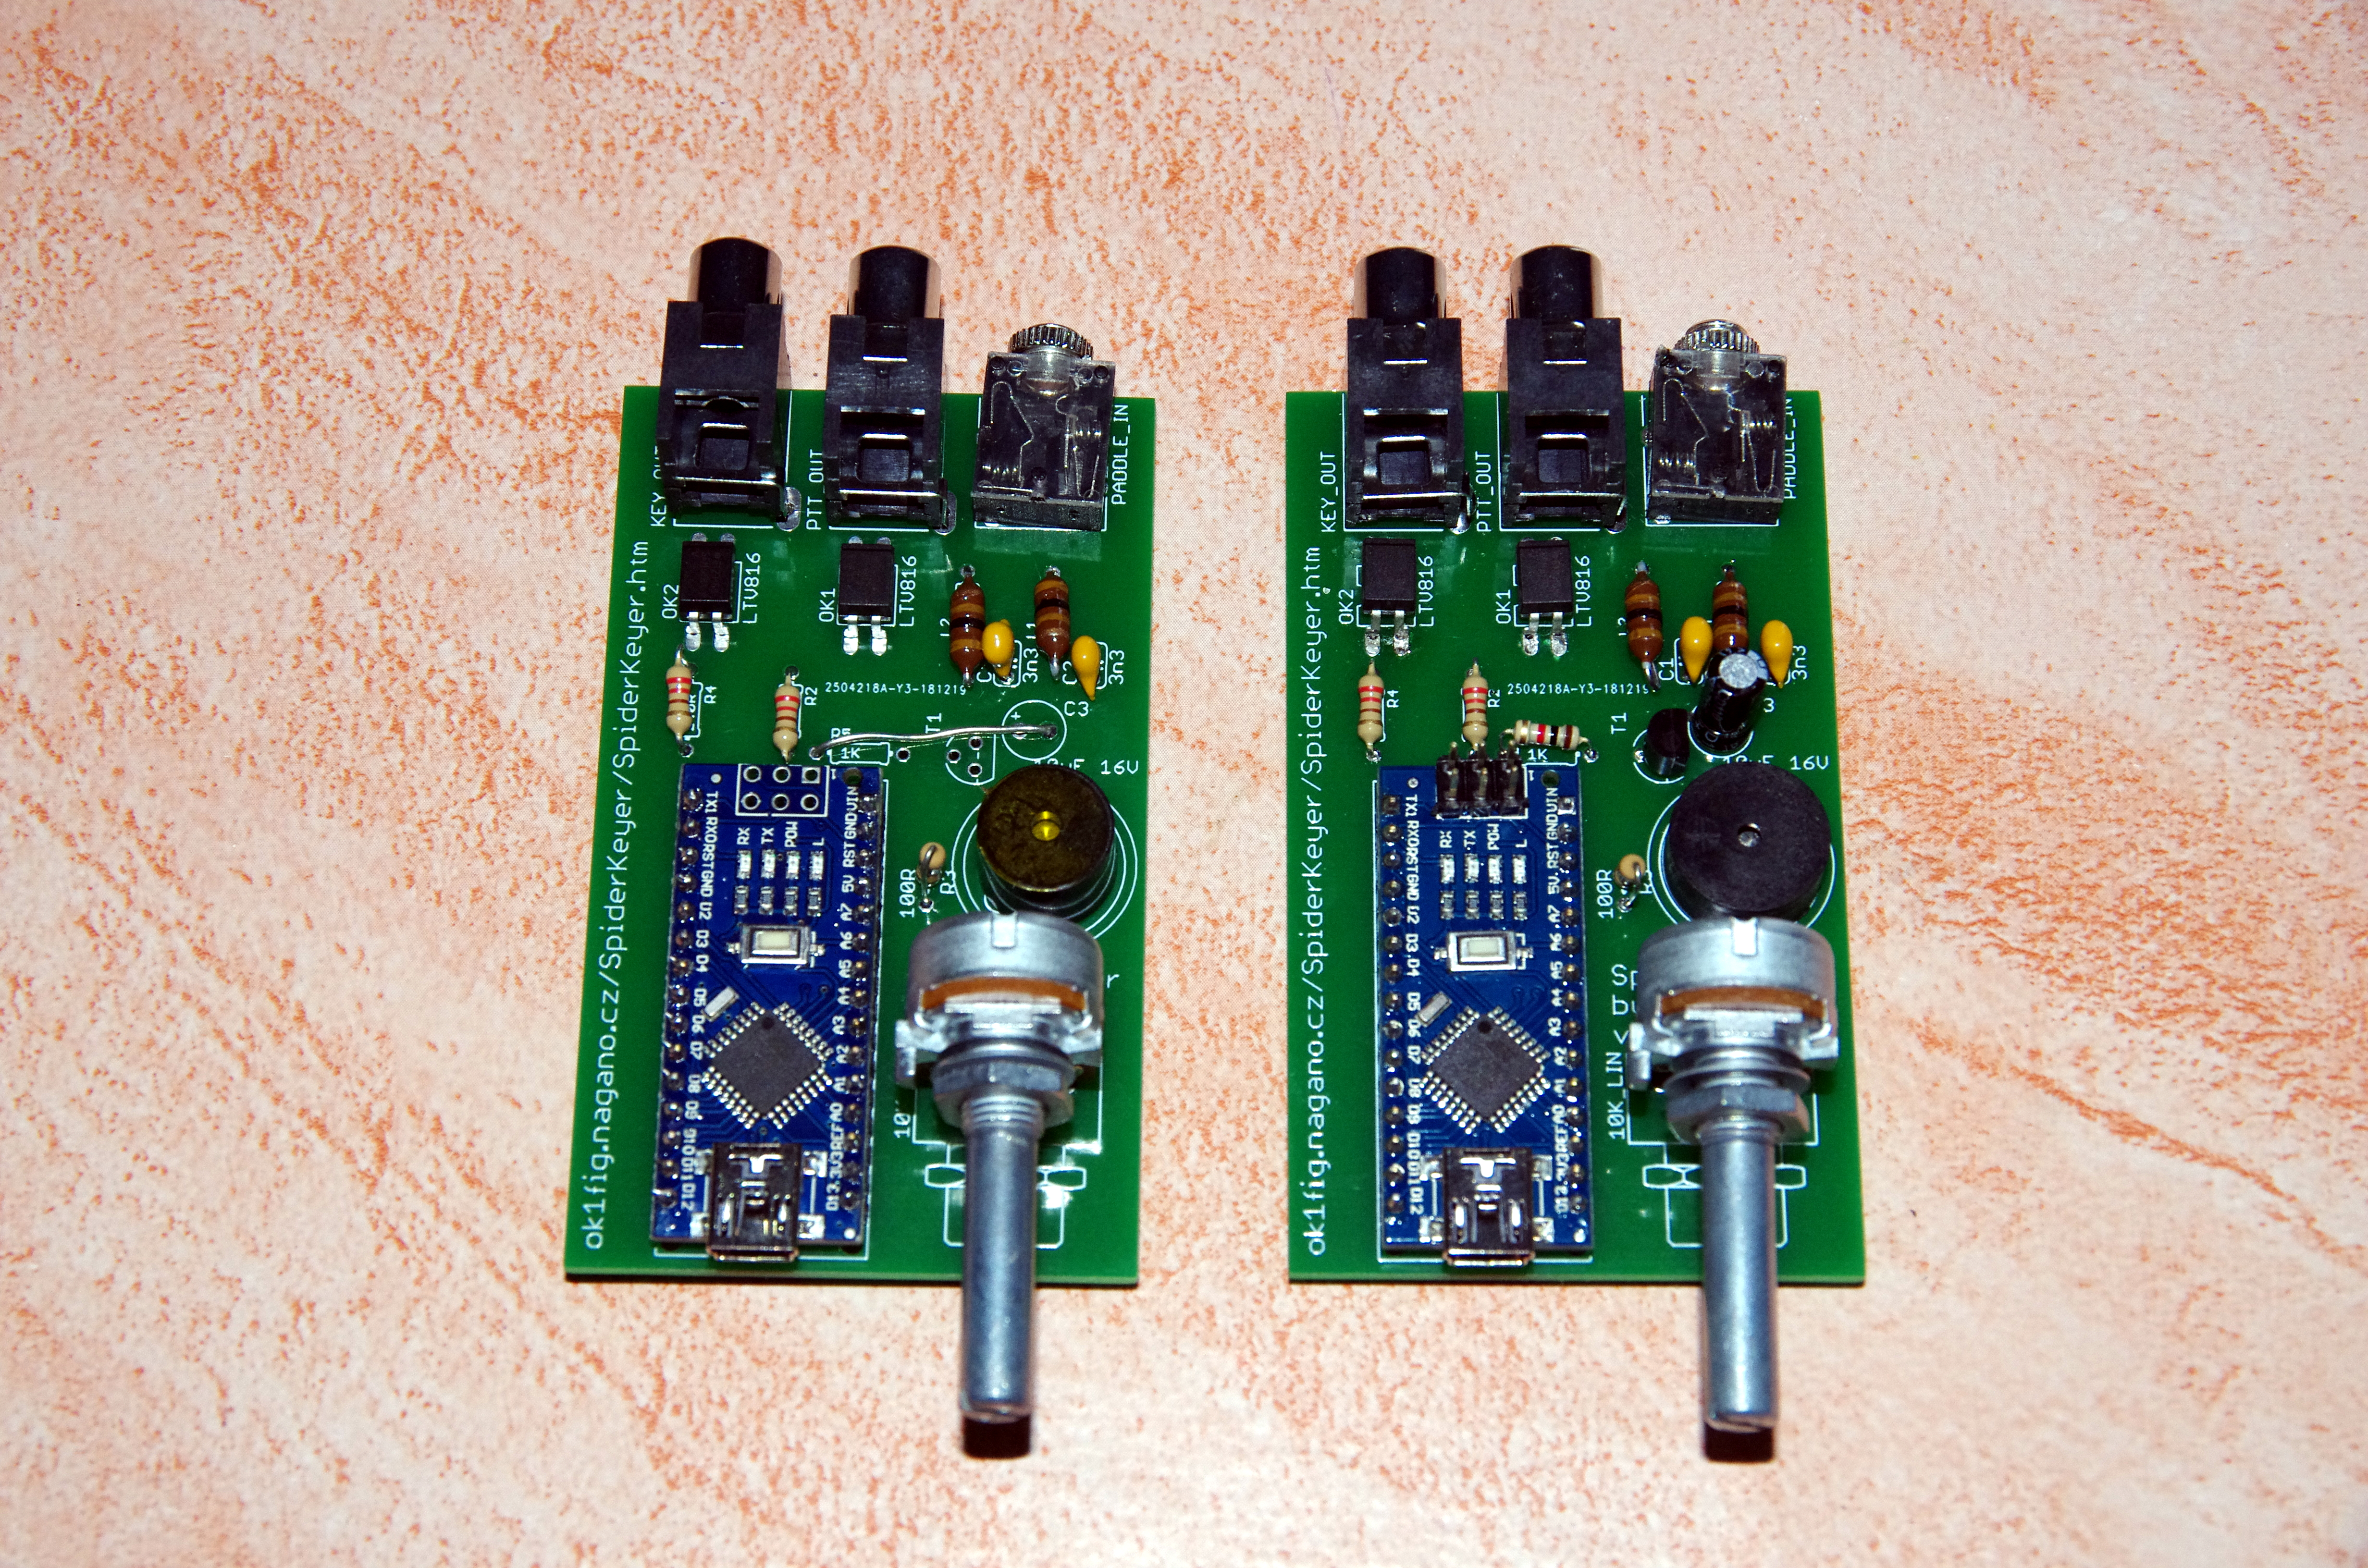
\includegraphics[width=\linewidth]{./IMGP4408.JPG}
	\end{center}
\end{samepage}
\pagebreak
\begin{samepage}
	Lo Spider Keyer pu\`o essere costruito su una breadboard o una millefori basandosi sullo schema (sezione \ref{sec:sch}), ma \`e consigliabile incidere la propria PCB per minimizzare il rischio di errori e avere un risultato pi\`u duraturo.
	\begin{center}
		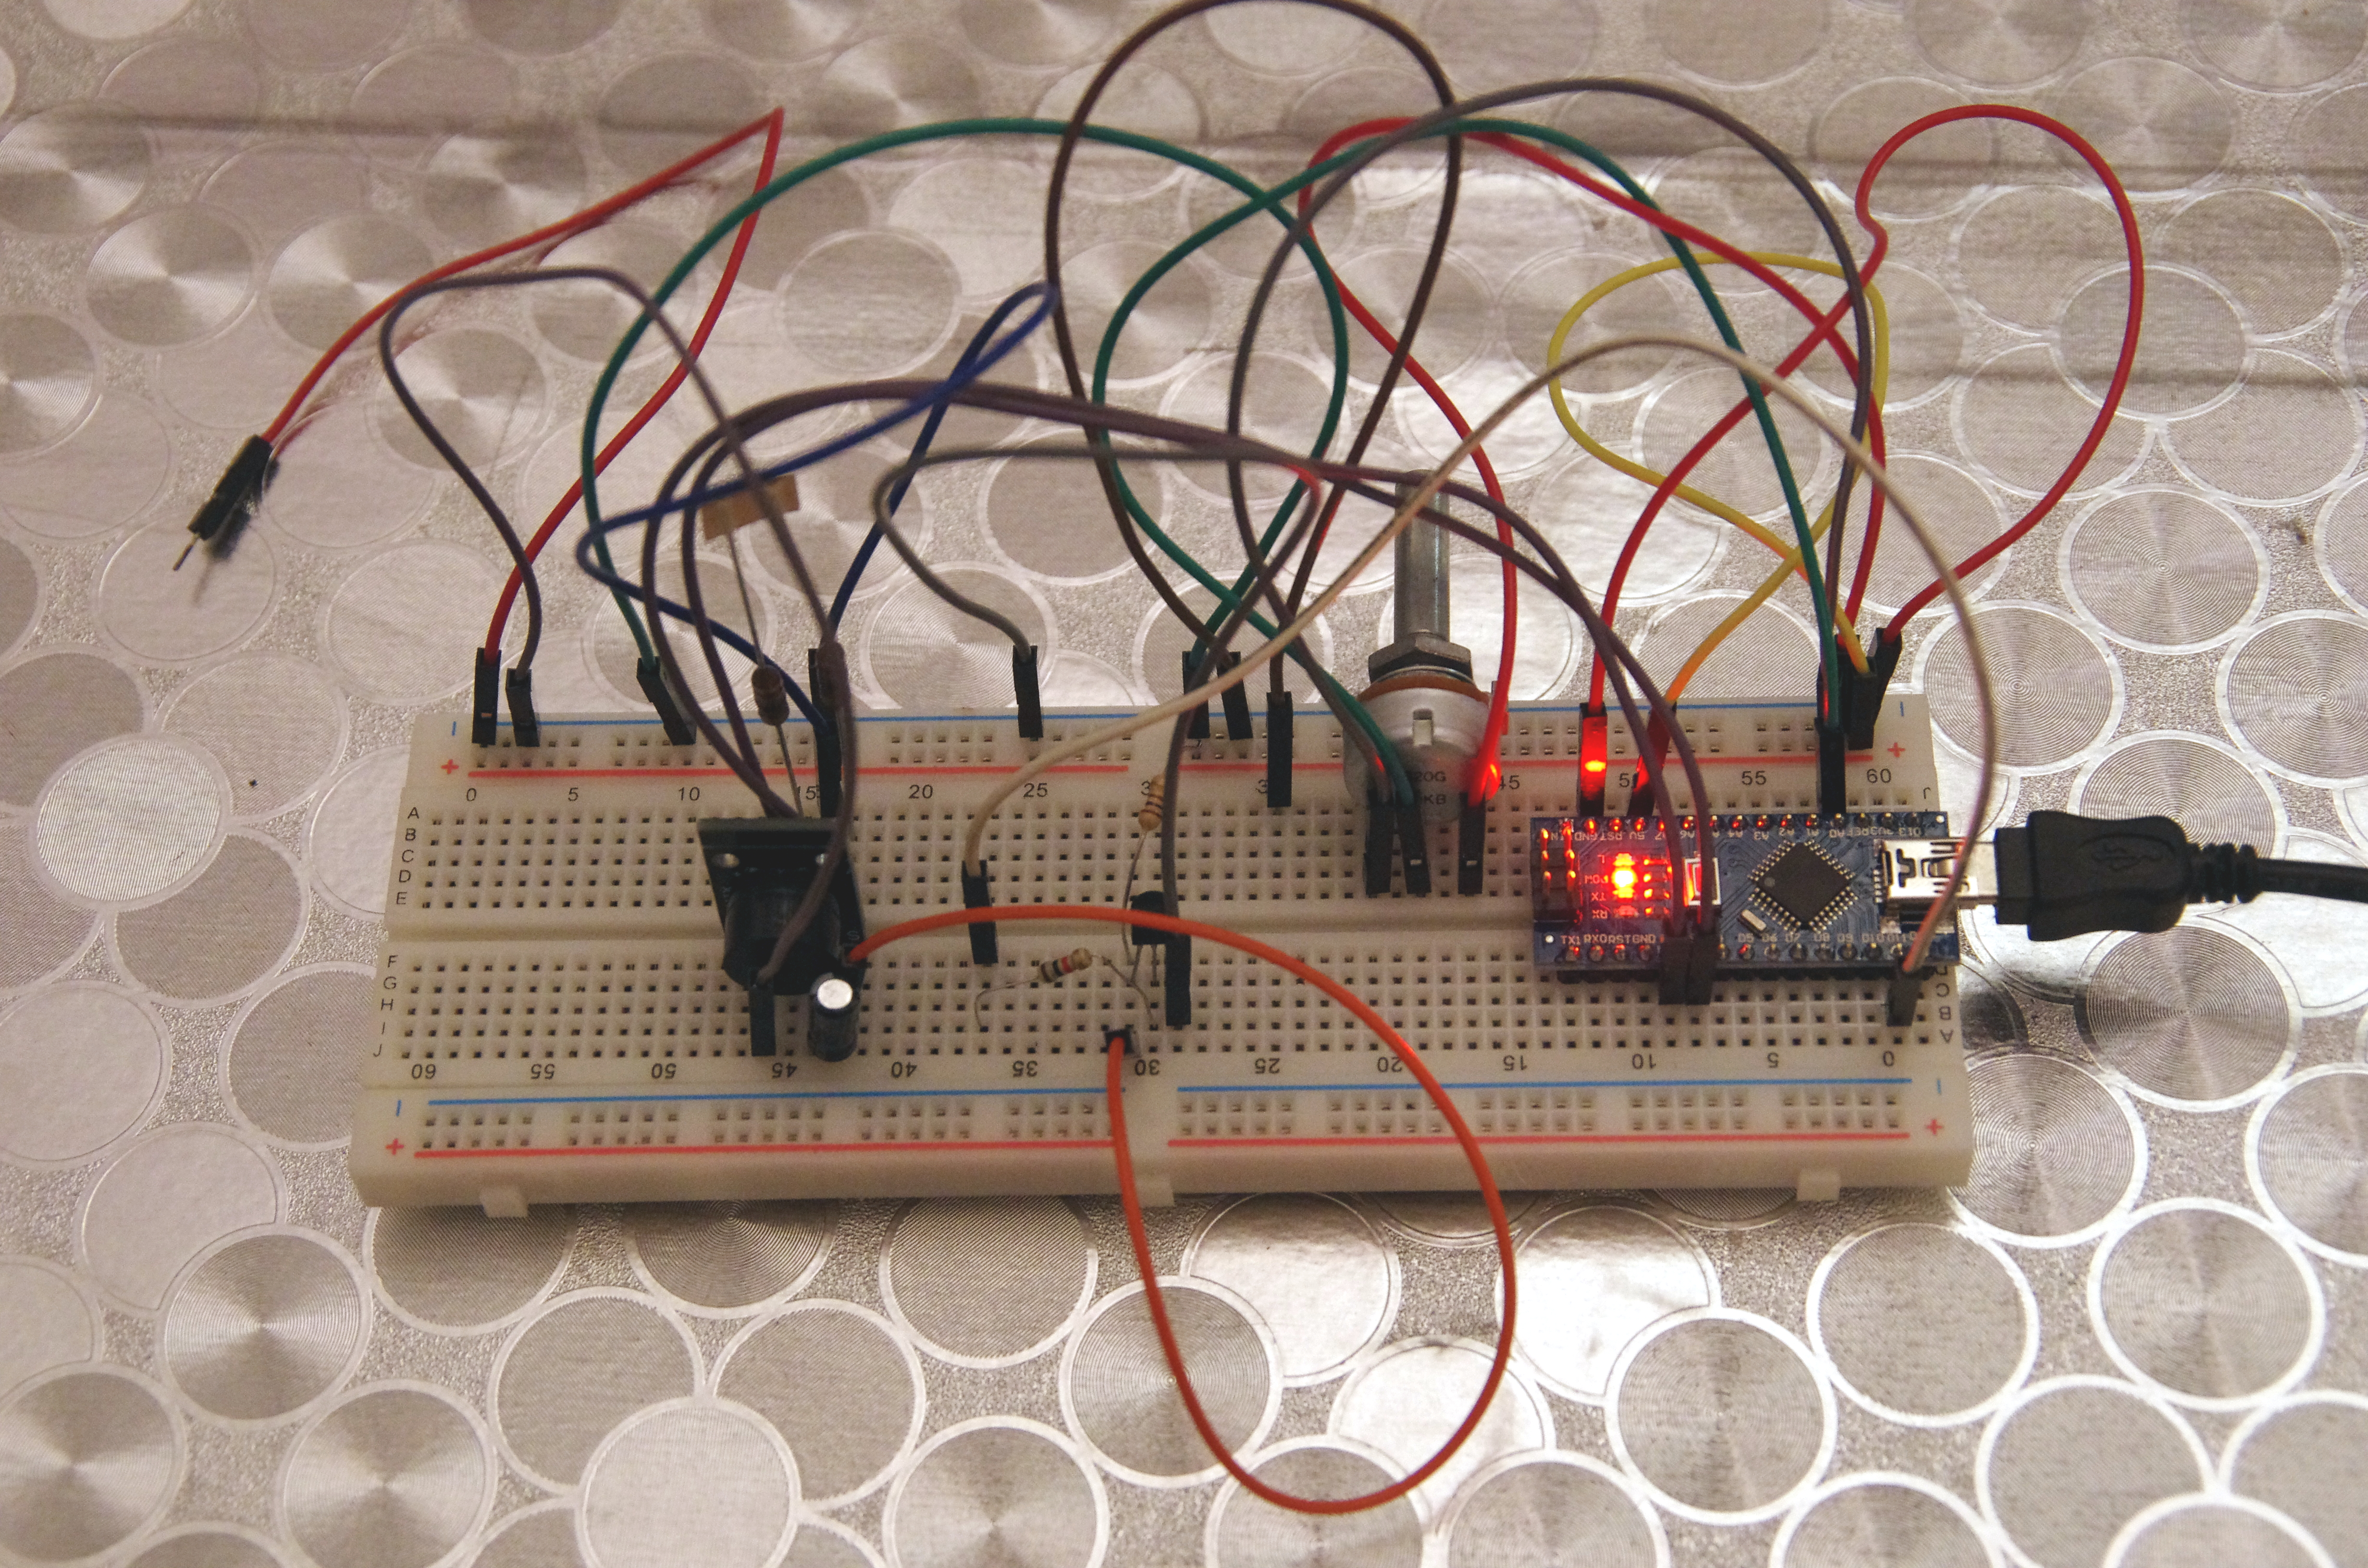
\includegraphics[width=\linewidth]{./bread.JPG}
		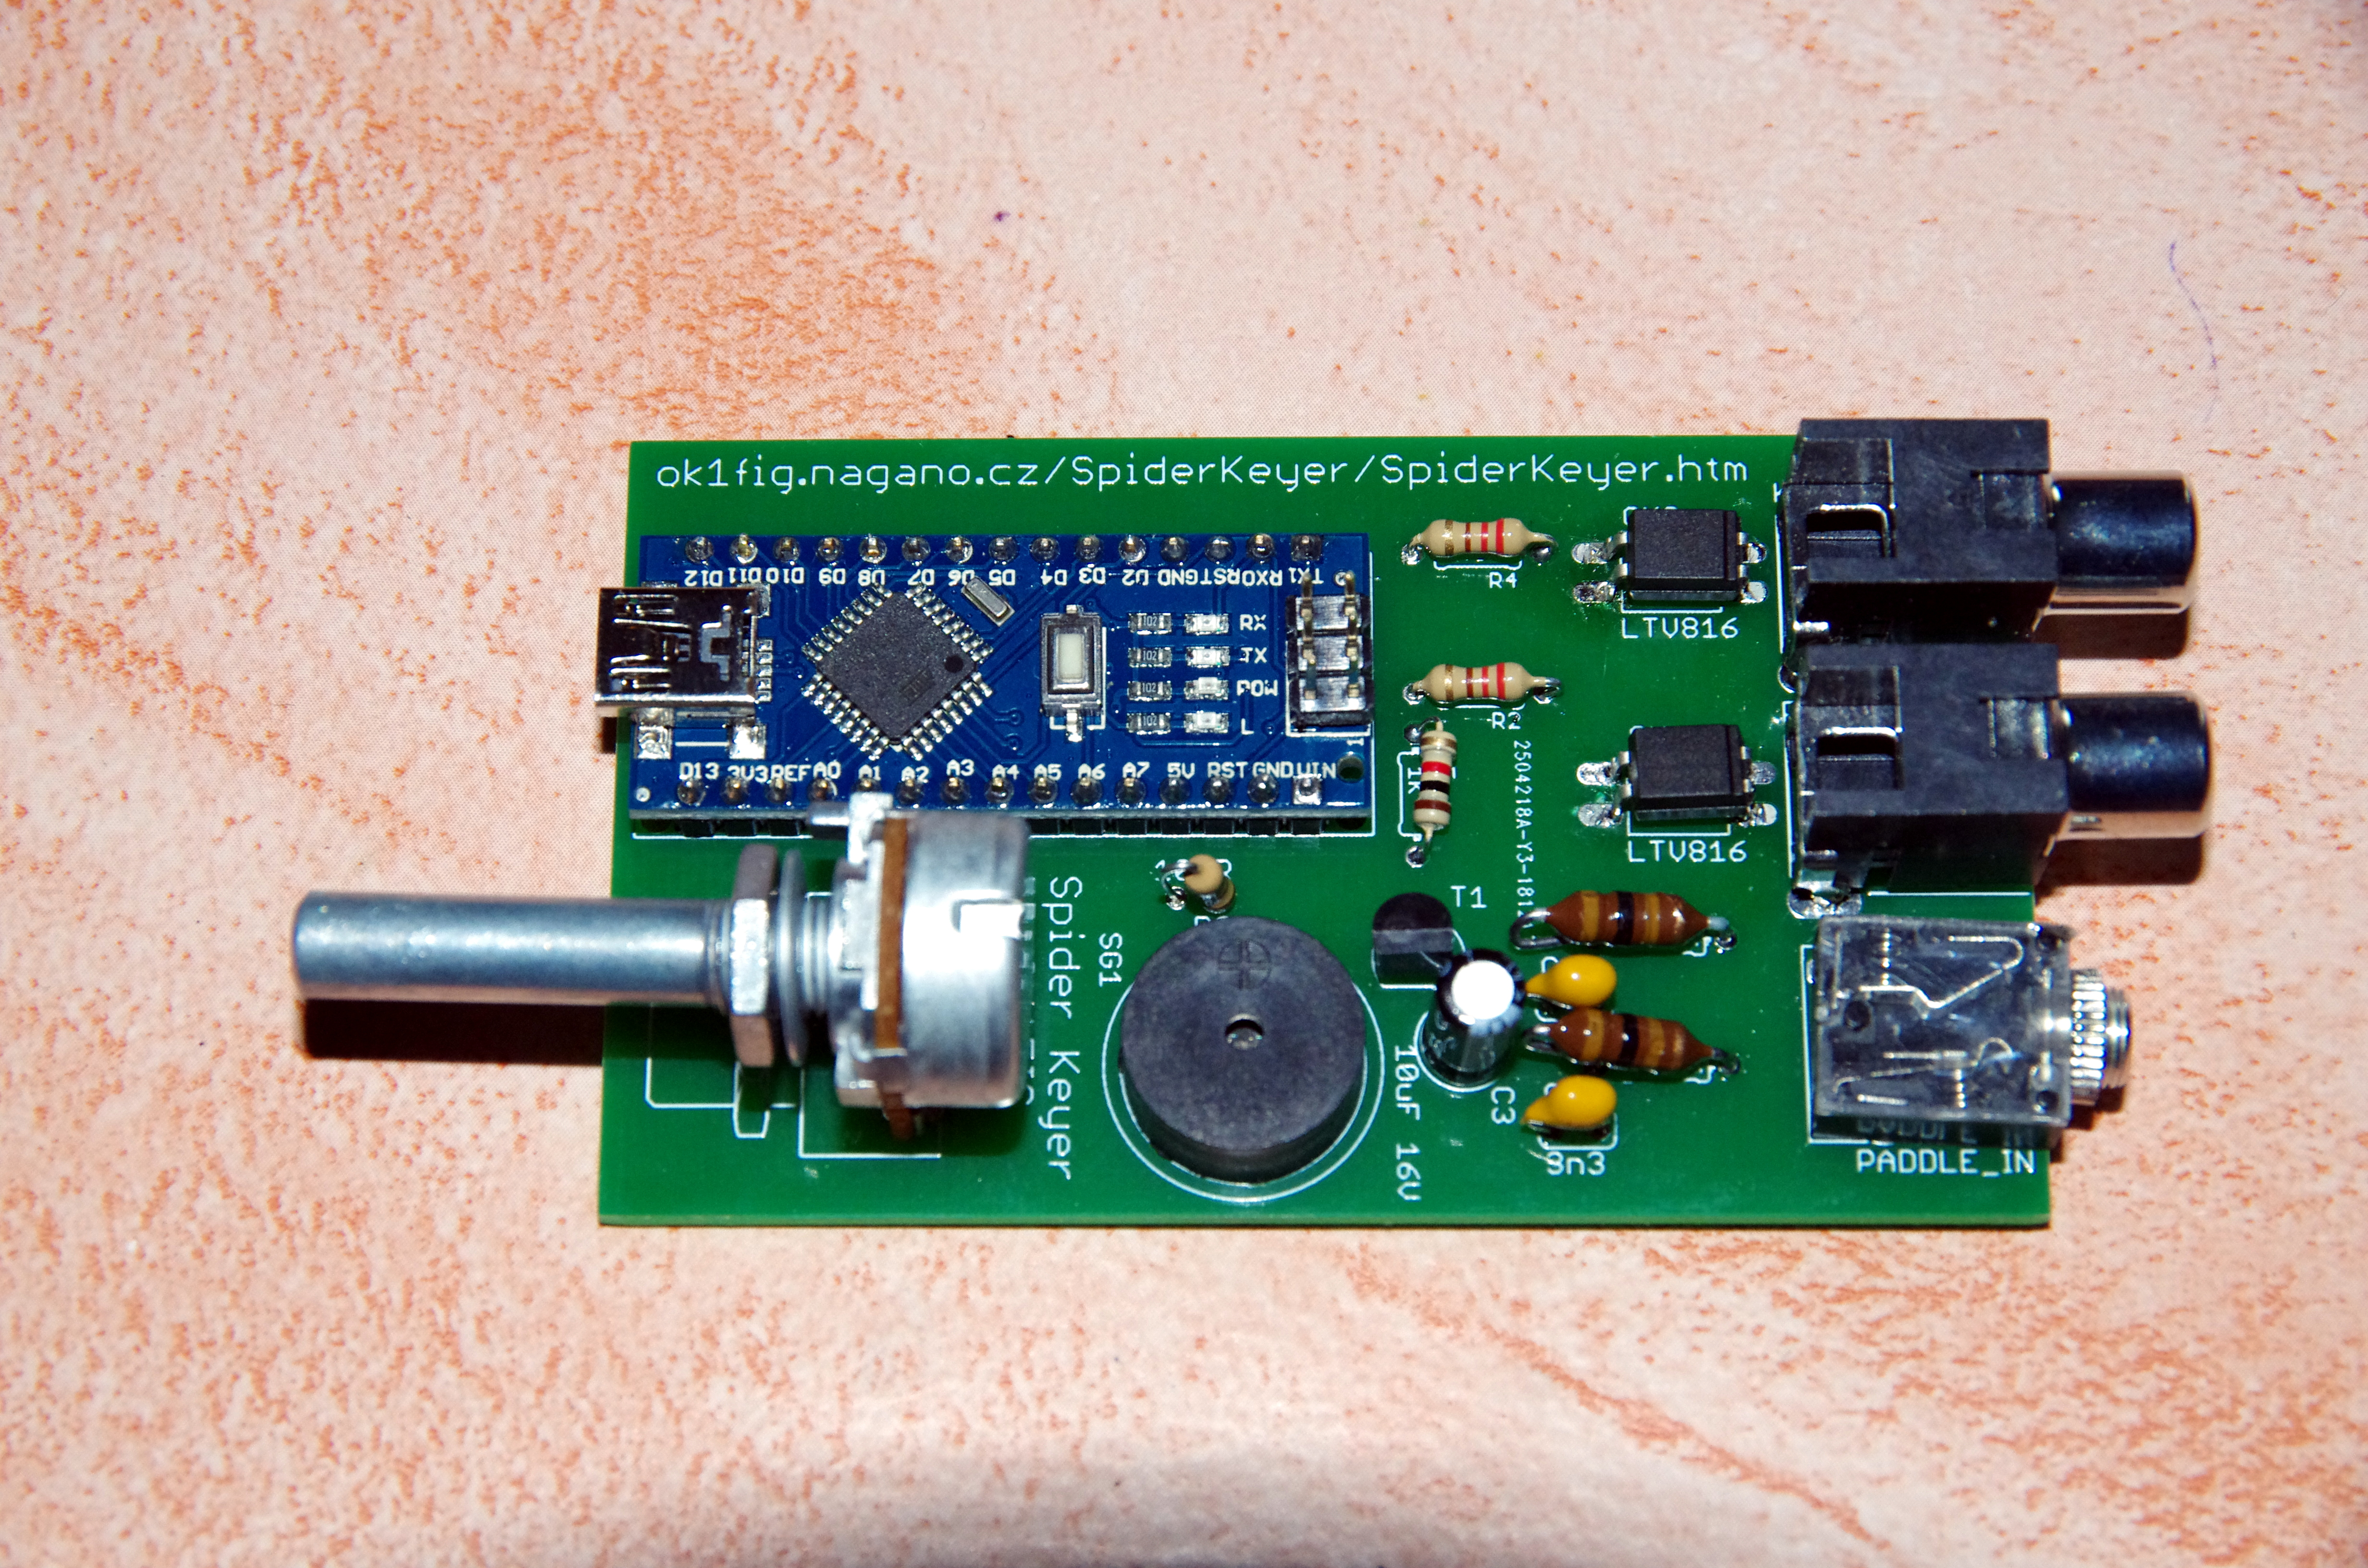
\includegraphics[width=\linewidth]{./IMGP4415.JPG}		
	\end{center}
	
\end{samepage}

\section{Schemi}\label{sec:sch}
\begin{center}
	\includegraphics[width=\linewidth]{./schema.png}
\end{center}

\begin{samepage}
	OK1FIG ha messo a disposizione sul sito i layout per incidere manualmente le PCB:
	\begin{center}
		\includegraphics[width=.5\linewidth]{./PCB_xray.png}\includegraphics[width=.5\linewidth]{./PCB_cuprum.png}
	\end{center}
\end{samepage}


\begin{samepage}
	Tuttavia, ho preferito riprogettare il circuito in formato Gerber per poter fare incidere pi\`u copie a una ditta specializzata (\url{jlcpcb.com}). Insieme a questo manuale sono presenti i file Gerber nell'archivio \texttt{SpiderKeyerGerber.zip}:
	\begin{center}
		\includegraphics[width=.5\linewidth]{./latorame.png}\includegraphics[width=.5\linewidth]{./latocomponenti.png}
	\end{center}
\end{samepage}


\section{Firmware}
Per poter funzionare correttamente, lo Spider Keyer deve essere programmato. Insieme a questo manuale \`e presente il codice sorgente nella cartella \texttt{SpiderKeyer} e l'IDE Arduino in un archivio zip.

\begin{enumerate}
	\item Dopo aver scompattato l'archivio \texttt{arduino-1.8.8-windows.zip}, connettere l'Arduino Nano al PC tramite cavo mini USB, e se necessario installare i driver dalla cartella \texttt{arduino-1.8.8-windows/drivers} (nel caso di cloni, sar\`a necessario scaricare driver diversi da quelli ufficiali: insieme a questo manuale sono presenti nell'archivio \texttt{Elegoo CH340 Driver 2018.11.27.zip} i driver per il clone ELEGOO Nano).
	\item Lanciare il programma \texttt{arduino.exe}:
	\begin{center}
		\includegraphics[width=\linewidth]{./firmware01.png}
	\end{center}
	\item Fare click su \texttt{File > Open...} e cercare il sorgente \texttt{SpiderKeyer.ino}:
	\begin{center}
		\includegraphics[width=\linewidth]{./firmware02.png}
	\end{center}
	\item Fare click su \texttt{Tools} e settare le impostazioni come:
	\begin{itemize}
		\item Board: \texttt{Arduino Nano}
		\item Processor: \texttt{ATmega328P} (nel caso di cloni come l'ELEGOO Nano potrebbe essere necessario selezionare \texttt{ATmega328P (Old Bootloader)})
		\item Port: quella a cui \`e connesso l'Arduino.
	\end{itemize}
	\begin{center}
		\includegraphics[width=\linewidth]{./firmware03.png}
	\end{center}
	\item Fare click sul tasto \texttt{Upload} e attendere la fine del caricamento:
	\begin{center}
		\includegraphics[width=\linewidth]{./firmware04.png}
	\end{center}
\end{enumerate}








